\section{Deep Learning Methods in Action Recognition}
META: Review of approaches that use Deep Learning.

\subsection{Spatio-Temporal Networks}
I.e. convolutional methods.

\subsubsection{3D Convolutional Neural Networks for Human Action Recognition -- Ji et al. (2013)}

In this work \cite{ji_3d_2013} the authors porpose 3D convolution for action recognition from video data, which processes spatial as well as temporal information in a convolutional layer.

In regular convolutional neural networks 2D convolutions are applied in the convolutional layers to extract features from the feature maps in the previous layer. More formally in the notation of the authors, the value of feature map $j$ in the $i$th layer at spatial position $(x,y)$ is given by:

\begin{align*}
    v_{ij}^{xy} = \tanh \left( b_{ij} + \sum_m \sum_{p=0}^{P_i -1} \sum_{q = 0}^{Q_i - 1} w_{ijm}^{pq} v_{(i-1)m}^{(x+p)(y+q)} \right)
\end{align*}

$w_{ijm}^{pq}$ denotes the value at position $(p,q)$ of the kernel, that performs convolution on feature map $m$ of the previous layer, resulting in feature map $j$ in layer $i$.
$P_i$ and $Q_i$ denote the dimensions of the kernel in x- and y-direction respectively.
Tensor $w$ therefore represents all kernels that produce the feature maps in layer $i$ through convolution.

The two inner sums carry out the convolutional operation on feature map $m$ of the previous layer, which is then combined with the results for the other feature maps by summation over $m$, added with a bias and fed into a non-linear function ($\tanh(\cdot)$) to result in the value of the current feature map.

Note: The convolutional operation used here is called cross-correlation, which differs from mathematical discrete convolutions in that the kernel is not flipped. This results in a non-commutative operation as described in chapter 9 of cite deep learning book ??

The authors propose an extension of 2D convolutions by using a three dimensional kernel. More formally, in the notation as above, the value of feature map $j$ in the $i$th layer at position $(x,y,z)$ is given by:

\begin{align*}
    v_{ij}^{xyz} = \tanh \left( b_{ij} + \sum_m \sum_{p=0}^{P_i -1} \sum_{q = 0}^{Q_i - 1} \sum_{r = 0}^{R_i - 1} w_{ijm}^{pqr} v_{(i-1)m}^{(x+p)(y+q)(z+r)} \right)
\end{align*}

As above, $w_{ijm}^{pqr}$ denotes the value of the now three dimensional kernel at position $(p,q,r)$, which performs convolution on the $m$th feature map of the previous layer.
$R_i$ denotes the dimension of the kernel in temporal direction. 

Based on the 3D convolution, the authors design a neural network architecture, that takes an input of 7 frames of size 60x40.

The network is evaluated as part of an action detection and recognition system on the TRECVID (TREC Video Retrieval Evaluation) data, which consists of surveillance videos recorded at London Gatwick Airport.

The details of the architecture are described below:

\begin{figure}[H]
    \centering
    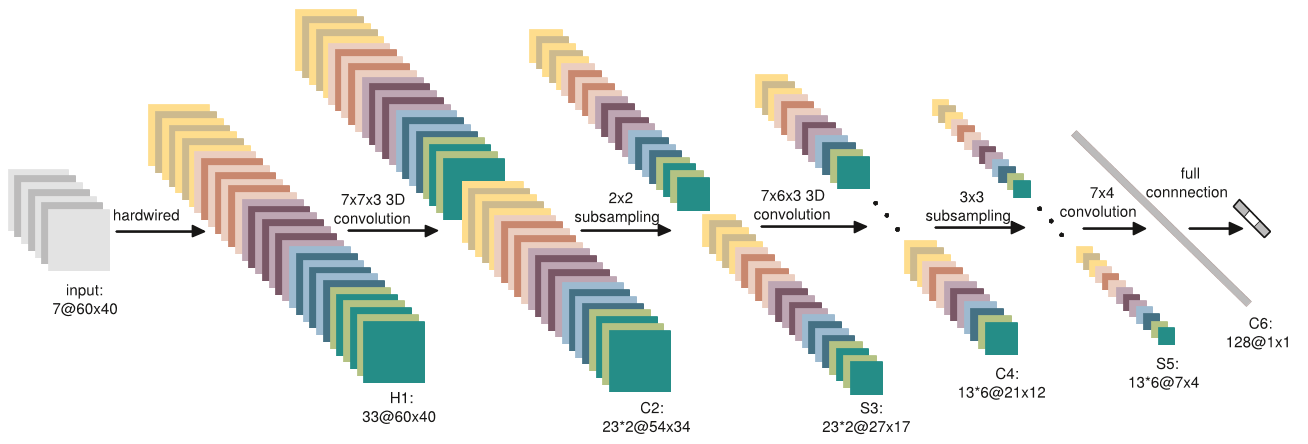
\includegraphics[width=\textwidth]{img_deep/3dconv_architecture}
    \caption{3D CNN architecture developed for human action recognition on the TRECVID 2008 development dataset \cite{ji_3d_2013}}
    \label{fig:3dconv_architecture}
\end{figure}

At first several hard wired kernels are applied to the input frames, which extract gray values, gradients along the horizontal and vertical direction in the frames and the optical flow between two consecutive frames. This results in 33 feature maps, organized in 5 different channels: gray, gradient-x, gradient-y, optflow-x and optflow-y.

In the first convolutional layer C2 two 3D kernels with dimesions 7x7x3 (7x7 in the spatial dimension and 3 in the temporal dimension) are applied at each of the five channels separately. 
The first convolutional layer therefore contains $2 \times 5 \times 7 \times 7 \times 3 \text{ (kernel-weights) } + 2 \times 5 \text{ (biases) } = 1480$ trainable parameters. 

After a subsampling layer S3, three different kernels are applied to each of the 2x5 channels of the previous layer.

The last convolutional layer performs 2D convolutions to obtain 128 feature maps of dimension 1x1.
These feature maps are a 128 dimensional vector representation of the input.

The resulting feature vector is then classified (in this task here into three different classes) by a fully connected layer.

The complete architecture has 295.458 trainable parameters in total, which are initialized randomly and learned by online error back-propagation. cite lecun 1998



\subsubsection{Large-scale Video Classification with Convolutional Neural Networks -- Karpathy et al. (2014)}

\subsection{Multiple Stream Networks}
The most successfull architecture at action recognition. They are equally powerful as the improved dense trajectories approach. cite TDD ??

These approaches use the decomposability of videos into a spatial component (analysing different frames) and a temporal component (analysing the change between frames) for action recognition.

The first architecture of this kind was proposed in 2014 from Simonyan and Zisserman.

\subsubsection{Two-Stream Convolutional Networks for Action Recognition in Videos - Simonyan and Zisserman (2014)}

The authors propose a novel architecture for action recognition with two separate recognition streams (spatial- and temporal-stream) which are combined by late fusion.

The authors evaluate two different fusion methods: building the average of both network's outputs and training a linear multi-class SVM on stacked $L_2$-normalised softmax scores.

This approach is motivated by the two-streams hypothesis cite (??), according to which the human visual cortex contains two paths: the ventral stream for object recognition and the dorsal stream for recognising motion.

Both streams are implemented as deep CNNs, with the rectification activation function for all hidden units.

\begin{figure}[H]
    \centering
    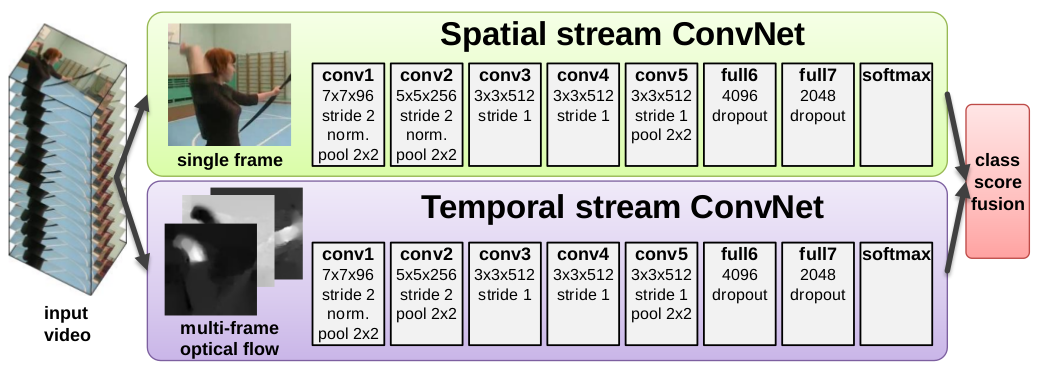
\includegraphics[width=0.9\textwidth]{img_deep/twostream_architecture}
    \caption{Two-stream architecture for video classification, depicting the spatial- and temporal-stream with implementation details as deep Convolutional Neural Network \cite{simonyan_two-stream_2014}}
    \label{fig:twostream_architecture}
\end{figure}

Spatial stream: Takes single video frames as input. Performs action recognition from still images and is fairly competitive on its own. Basically an image recognition architecture. Advantage: Can be pre-trained using large amount of image data, here from the ImageNet challenge dataset cite (??).

Spatial part of a video, i.e. the individual static frames, convey information about the objects and persons in the scene.

Temporal stream: is trained to recognize actions from motions given in the form of dense optical flow.

The temporal part of a video, i.e. the change between frames, conveys information about the movement of the observer (camera) and the movement of objects in the scene.

The second normalisation layer was removed from the the temporal stream network in order to reduce memory usage.

The authors propose two methods for constructing the input to the temporal network by stacking optical flow displacement fields along several consecutive frames of the input video.

\textbf{Optical Flow Stacking:} \\
A dense optical flow field $\mathbf{d}_t(u,v)$ of two consecutive frames at times $t$ and $t+1$ can be thought of as a two dimensional vector-field, which maps the displacement of each pixel along the transition from frame $t$ to $t+1$. In this case $u,v \in \mathbb{N}$, $1 \leq u \leq w$ and $1 \leq v \leq h$ where $w$ and $h$ are the width and height of the video frames.

The horizontal and vertical components $d_t^x(u,v)$, $d_t^y(u,v)$ can be interpreted as image channels.

This method constructs the input volume $I_\tau \in \mathbb{R}^{w \times h \times 2L}$ of the temporal stream network by stacking the horizontal and vertical components of the dense optical flow field along $L$ consecutive frames, beginning at time $\tau$. Formally, with $1 \leq k \leq L$:
\begin{align*}
    I_\tau(u,v,2k-1) = d_{\tau + k - 1}^x(u,v) \\
    I_\tau(u,v,2k) = d_{\tau + k - 1}^{y}(u,v)
\end{align*}

\textbf{Trajectory Stacking:} \\
Instead of sampling at fixed locations in each frame, this methods samples the dense optical flow field along the motion trajectories of the initial points in frame $\tau$.

Let $\mathbf{p}_k$ denote the motion trajectory of initial point $(u,v)$. With $1 < k \leq L$ and \mbox{$\mathbf{p}_1 = (u,v)$} the trajectory is recursively defined by:
\begin{align*}
    \mathbf{p}_k = \mathbf{p}_{k-1} + \mathbf{d}_{\tau + k - 2}(\mathbf{p}_{k-1})
\end{align*}

The input volume can then be constructed by sampling the horizontal and vertical optical flow components along these trajectories.

\begin{align*}
    I_\tau(u,v,2k-1) = d_{\tau + k - 1}^x(\mathbf{p}_{k}) \\
    I_\tau(u,v,2k) = d_{\tau + k - 1}^y(\mathbf{p}_{k})
\end{align*}

\begin{figure}[H]
    \centering
    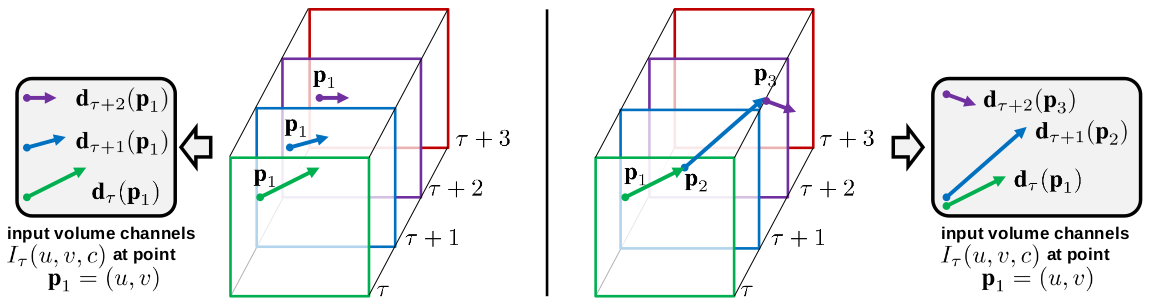
\includegraphics[width=0.9\textwidth]{img_deep/trajectory_stacking}
    \caption{Construction of input volumes from multi-frame optical flow. Left: Optical Flow Stacking. Right: Trajectory Stacking \cite{simonyan_two-stream_2014}}
    \label{fig:trajectory_stacking}
\end{figure}

Since the Convolutional Networks require fixed sized inputs, the authors sample a $224 \times 224 \times 2L$ subvolume from $I_\tau \in \mathbb{R}^{w \times h \times 2L}$ and use it as the temporal networks input.

By using optical flow, the authors explicitly incorporate a representation of motion in their action recognition architecture.

The authors further describe two optional techniques that are evaluated for constructing the inputs with either one of optical flow stacking methods.
\begin{enumerate}
    \item \textbf{Bi-directional Optical Flow}: The input volume $I_{\tau}$ is created by using regular forward optical flow from frame $\tau$ to $\tau + L/2$ and additionally calculated optical flow from frame $\tau$ to $\tau - L/2$ in the backwards direction. Stacking the horizontal and vertical components of these optical flow fields results in an input volume of length $L/2$ around frame $\tau$ in both directions. 
    \item \textbf{Mean flow subtraction}: The displacement vectors between two frames can dominantly be caused by global movement of the camera. Compared to regular camera-motion compensation, the authors use a simpler approach and just subtract the mean vector from each displacement field $\mathbf{d}_t$.
\end{enumerate}

An advantage of separating the spatial and the temporal stream is the possibility of pre-training the spatial net with large pre-existing image datasets (here ImageNet ILSVRC-2012 ??).

For training the temporal stream network with video-data, the authors address the general problem of video action recognition, that the existing datasets are too small in comparison to their image-dataset counterparts.

The authors use, according to the multi-task learning paradigm \cite{collobert_unified_2008}, the UCF-101 and the HMDB-51 dataset simultaneously for training the temporal stream network (see chapter ??). 

By training a network on several tasks (here UCF-101 classification and HMDB-51 classification), the network learns more general video representations, since the second task acts as regulariser and more data can be utilized.

The authors implement this by using two softmax classification layers, one for each dataset. Each softmax layer has its own loss function and the sum of the individual losses is taken as the overall training loss for computing the weight updates by backpropagation.

Training for both networks is conducted with mini-batch gradient descent with 256 randomly selected videos at each iteration. From each of those videos, a single frame is randomly chosen, a $224 \times 224$ sub-image is randomly cropped, randomly horizontal flipped, RGB jittered and then used as training input for the spatial stream network.

An optical flow volume is constructed for this selected frame as described above. For optical flow computation the authors use a fast implementation (0.06s per pair of frames) from the OpenCV toolbox. Despite it's speed, on-the-fly computation of optical-flow would be a bottleneck and is therefore pre-computed and stored for the complete datasets.

The creators of UCF-101 and HMDB-51 provide three splits of their datasets into training- and testing-data. The standard evaluation procedure is to report the average accuracy over those three splits, which the authors follow in this work as well.

The authors build their final design of the two-stream architecture by evaluating different setups for the spatial and temporal stream network on their own using UCF-101 (split 1).

Besides using two different dropout rate (0.5 and 0.9), the performance of the spatial-stream network is evaluated for:
\begin{enumerate}
    \item Training the complete network from scratch on UCF-101.
    \item Pre-training the network on ILSVRC-2012 and fine-tuning it on UCF-101.
    \item Pre-training the network on ILSVRC-2012 and fine-tuning of only the last (classification) layer.
\end{enumerate}

For evaluating the temporal-stream network a fixed dropout rate of 0.9 is chosen, because the network needs to be trained from scratch. The performance is then measured for:
\begin{enumerate}
    \item Using one or several (stacked) optical flow displacement fields $L \in {1,5,10}$.
    \item Regular optical flow stacking
    \item Trajectory stacking
    \item Using bi-directional optical flow
    \item Using mean subtraction
\end{enumerate}

The findings are presented in table \ref{tab:twostream_archeval}.

Spatial-stream network: The authors decided on pre-trained the network on ILSVRC and fine-tuning only the last layer.

Temporal-stream network: Mean subtraction and stacking multiple optical flows is beneficial, so $L=10$ is used as the default setting. Regular optical flow stacking performs better than trajectory stacking and bi-directional optical flow only yields slight improvement against forward optical flow. Therefore regular forwars optical flow stacking is chosen for the temporal-stream network.

The authors highlight that the temporal-stream network significantly outperforms the spatial-stream network, which confirms the importance of motion information for action recognition from video.

\begin{table}[H]
    \centering
    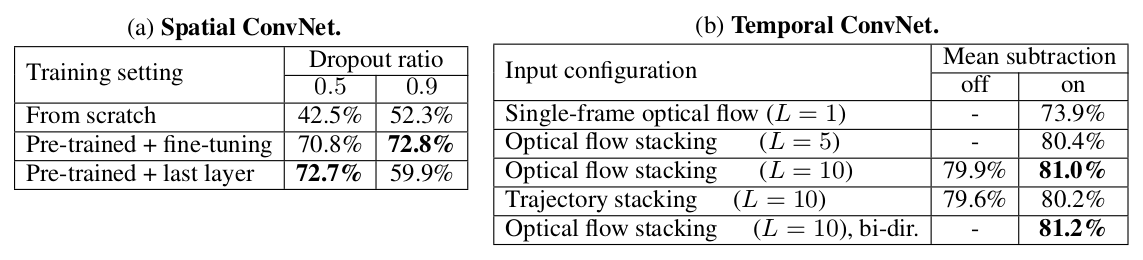
\includegraphics[width=\textwidth]{img_deep/twostream_archeval}
    \caption{Performance of the individual convolutional networks on UCF-101 (split 1) \cite{simonyan_two-stream_2014}}
    \label{tab:twostream_archeval}
\end{table}

After having found the optimal configurations for the individual temporal-stream and spatial-stream networks, the authors evaluate different fusion methods (averaging and SVM) and find that fusion by SVM performs best. The fused network's performance significantly improves over the individual network's performance, which implies, that the spatial and temporal recognition stream are complementary.

\begin{table}
    \centering
    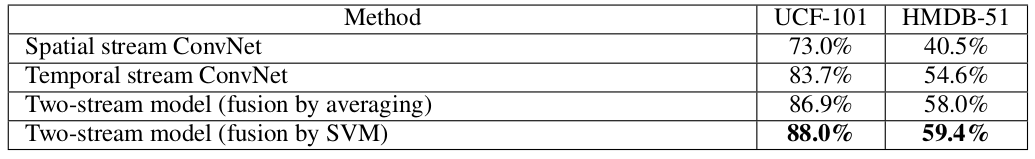
\includegraphics[width=\textwidth]{img_deep/twostream_results}
    \caption{Mean accuracy over three splits on UCF-101 and HMDB-51 \cite{simonyan_two-stream_2014}}
    \label{tab:twostream_results}
\end{table}

The results in table \ref{tab:twostream_results} show, that fusion by SVM works best.

\subsubsection{Action recognition with trajectory-pooled deep-convolutional descriptors -- Wang et al. (2014)}

\subsubsection{Fusing Multi-Stream Deep Networks for Video Classification -- Wu et al. (2015)}

\subsection{Generative Models}
Restricted Boltzmann Machine

\subsection{Temporal Coherency Networks}
